\documentclass[12pt,addpoints]{exam}
%-----------------------------------------------------------------------------
% PACKAGES AND OTHER DOCUMENT CONFIGURATIONS
%-----------------------------------------------------------------------------

\usepackage[margin=1in]{geometry}
\usepackage{amsmath, amsfonts}
\usepackage{enumerate}
\usepackage{graphicx}
\usepackage{titling}
\usepackage{url}
\usepackage{xfrac}
\usepackage{natbib}
\usepackage{amssymb}
\usepackage{amsthm}
\usepackage{paralist}
\usepackage{epstopdf}
\usepackage{tabularx}
\usepackage{longtable}
\usepackage{multirow}
\usepackage{multicol}
\usepackage[colorlinks=true,urlcolor=blue]{hyperref}
\usepackage{algorithm}
\usepackage{algorithmicx}
\usepackage[noend]{algpseudocode}
\usepackage{float}
\usepackage{enumerate}
\usepackage{array}
\usepackage{environ}
\usepackage{times}
\usepackage{textcomp}
\usepackage{caption}
\usepackage{parskip} % For NIPS style paragraphs.
\usepackage[compact]{titlesec} % Less whitespace around titles
\usepackage[inline]{enumitem} % For inline enumerate* and itemize*
\usepackage{datetime}
\usepackage{comment}
% \usepackage{minted}
\usepackage{lastpage}
\usepackage{color}
% \usepackage{xcolor}
\usepackage[dvipsnames]{xcolor}
\usepackage[final]{listings}
\usepackage{tikz}
\usetikzlibrary{shapes,decorations}
\usepackage{framed}
\usepackage{booktabs}
\usepackage{cprotect}
\usepackage{verbatimbox}
\usepackage{multicol}
\usepackage{hyperref}
\usepackage{subcaption}
\usepackage{mathtools} % For drcases
\usepackage{cancel}
\usepackage[many]{tcolorbox}
\tcbuselibrary{listings} % For listings within tcolorbox
\usepackage{soul}
\usepackage[bottom]{footmisc}
\usepackage{bm}
\usepackage{wasysym}
\usepackage{lipsum}

\usepackage{tikz}
\usetikzlibrary{arrows}
\usetikzlibrary{arrows.meta}
\usetikzlibrary{shapes.geometric}
\usetikzlibrary{positioning, arrows, automata, calc}
\usepackage{transparent}
\usepackage{tikz-cd}

%%%%%%%%%%%%%%%%%%%%%%%%%%%%%%%%%%%%%%%%%%%
% Formatting for \CorrectChoice of "exam" %
%%%%%%%%%%%%%%%%%%%%%%%%%%%%%%%%%%%%%%%%%%%

\CorrectChoiceEmphasis{}
\checkedchar{\blackcircle}

\newenvironment{checkboxessquare}{
    \begingroup
    \checkboxchar{$\Box$} \checkedchar{$\blacksquare$} % change checkbox style locally
    \begin{checkboxes}
    }{
    \end{checkboxes}
    \endgroup
    }

    
\newenvironment{oneparcheckboxessquare}{
    \begingroup
    \checkboxchar{$\Box$} \checkedchar{$\blacksquare$} % change checkbox style locally
    \begin{oneparcheckboxes}
    }{
    \end{oneparcheckboxes}
    \endgroup
    }

%%%%%%%%%%%%%%%%%%%%%%%%%%%%%%%%%%%%%%%%%%%
% Better numbering                        %
%%%%%%%%%%%%%%%%%%%%%%%%%%%%%%%%%%%%%%%%%%%

% \numberwithin{equation}{section} % Number equations within sections (i.e. 1.1, 1.2, 2.1, 2.2 instead of 1, 2, 3, 4)
% \numberwithin{figure}{section} % Number figures within sections (i.e. 1.1, 1.2, 2.1, 2.2 instead of 1, 2, 3, 4)
% \numberwithin{table}{section} % Number tables within sections (i.e. 1.1, 1.2, 2.1, 2.2 instead of 1, 2, 3, 4)

%%%%%%%%%%%%%%%%%%%%%%%%%%%%%%%%%%%%%%%%%%
% Custom commands                        %
%%%%%%%%%%%%%%%%%%%%%%%%%%%%%%%%%%%%%%%%%%
\newcommand{\blackcircle}{\tikz\draw[black,fill=black] (0,0) circle (1ex);}
\renewcommand{\circle}{\tikz\draw[black] (0,0) circle (1ex);}

\newcommand{\solo}{ \textcolor{orange}{[SOLO]} }
\newcommand{\open}{ \textcolor{blue}{[OPEN]} }

\input{../shared/mathabbreviations.tex}

%%%%%%%%%%%%%%%%%%%%%%%%%%%%%%%%%%%%%%%%%%%
% Code highlighting with listings         %
%%%%%%%%%%%%%%%%%%%%%%%%%%%%%%%%%%%%%%%%%%%

\definecolor{bluekeywords}{rgb}{0.13,0.13,1}
\definecolor{greencomments}{rgb}{0,0.5,0}
\definecolor{redstrings}{rgb}{0.9,0,0}
\definecolor{light-gray}{gray}{0.95}

\newcommand{\MYhref}[3][blue]{\href{#2}{\color{#1}{#3}}}%

\definecolor{dkgreen}{rgb}{0,0.6,0}
\definecolor{gray}{rgb}{0.5,0.5,0.5}
\definecolor{mauve}{rgb}{0.58,0,0.82}

\lstdefinelanguage{Shell}{
  keywords={tar, cd, make},
  %keywordstyle=\color{bluekeywords}\bfseries,
  alsoletter={+},
  ndkeywords={python3, python, py, javac, java, gcc, c, g++, cpp, .txt, octave, m, .tar},
  %ndkeywordstyle=\color{bluekeywords}\bfseries,
  identifierstyle=\color{black},
  sensitive=false,
  comment=[l]{//},
  morecomment=[s]{/*}{*/},
  commentstyle=\color{purple}\ttfamily,
  %stringstyle=\color{red}\ttfamily,
  morestring=[b]',
  morestring=[b]",
  backgroundcolor = \color{light-gray}
}

\lstset{columns=fixed, basicstyle=\ttfamily,
    backgroundcolor=\color{light-gray},xleftmargin=0.5cm,frame=tlbr,framesep=4pt,framerule=0pt}

\newcommand{\emptysquare}{{\LARGE $\square$}\ \ }
\newcommand{\filledsquare}{{\LARGE $\boxtimes$}\ \ }
\def \ifempty#1{\def\temp{#1} \ifx\temp\empty }


% \newcommand{\squaresolutionspace}[2][\emptysquare]{\newline #1}{#2}
\def \squaresolutionspace#1{ \ifempty{#1} \emptysquare \else #1\hspace{0.75pt}\fi}
\newcommand{\squaresoln}[0]{ \begin{soln}\filledsquare \end{soln}}


\newcommand{\emptycircle}{{\LARGE $\fullmoon$}\ \ }
\newcommand{\filledcircle}{{\LARGE $\newmoon$}\ \ }
\def \circlesolutionspace#1{ \ifempty{#1} \emptycircle \else #1\hspace{0.75pt}\fi}
\newcommand{\circlesoln}[0]{ \begin{soln}\filledcircle \end{soln}}
%%%%%%%%%%%%%%%%%%%%%%%%%%%%%%%%%%%%%%%%%%%
% Custom box for highlights               %
%%%%%%%%%%%%%%%%%%%%%%%%%%%%%%%%%%%%%%%%%%%

% Define box and box title style
\tikzstyle{mybox} = [fill=blue!10, very thick,
    rectangle, rounded corners, inner sep=1em, inner ysep=1em]

% \newcommand{\notebox}[1]{
% \begin{tikzpicture}
% \node [mybox] (box){%
%     \begin{minipage}{\textwidth}
%     #1
%     \end{minipage}
% };
% \end{tikzpicture}%
% }

\NewEnviron{notebox}{

\begin{tikzpicture}
\node [mybox] (box){
    \begin{minipage}{0.95\textwidth}
        \BODY
    \end{minipage}
};
\end{tikzpicture}
}

%%%%%%%%%%%%%%%%%%%%%%%%%%%%%%%%%%%%%%%%%%%
% Commands showing / hiding solutions     %
%%%%%%%%%%%%%%%%%%%%%%%%%%%%%%%%%%%%%%%%%%%
\newcommand{\solutionspace}[4]{\fbox{\begin{minipage}[t][#1][t]{#2} \textbf{#3} \solution{}{#4} \end{minipage}}}

% To HIDE SOLUTIONS, set this value to 0:
%\providecommand{\issoln}{0}
%\providecommand{\issoln}{1}

\ifthenelse{\equal{\issoln}{1}}{

% SOLUTION environment
\newenvironment{soln}{\leavevmode\color{red}\ignorespaces }{}

% QUESTION AUTHORS environment
\newenvironment{qauthor}{\leavevmode\color{blue}\ignorespaces }{}

% Question tester comment environment
\newenvironment{qtester}{\leavevmode\color{green}\ignorespaces}{}

% Question learning objective comment environment
\newenvironment{qlearningobjective}{\leavevmode\color{green}\ignorespaces}{}

}{ % ELSE

  \NewEnviron{soln}{}
  \NewEnviron{qauthor}{}
  \NewEnviron{qtester}{}
  \NewEnviron{qlearningobjective}{}

}

%% To HIDE TAGS set this value to 0:
\def\showtags{0}
%%%%%%%%%%%%%%%%
\ifcsname showtags\endcsname \else \def\showtags{1} \fi
% Default to an empty tags environ.
\NewEnviron{tags}{}{}
\if\showtags 1
% Otherwise, include solutions as below.
\RenewEnviron{tags}{
    \fbox{
    \leavevmode\color{blue}\ignorespaces
    \textbf{TAGS:} \texttt{\url{\BODY}}
    }
    \vspace{-.5em}
}{}
\fi

\newtcolorbox[]{answer_box}[1][]
{
    % breakable,
    fit,
    enhanced,
    % nobeforeafter,
    colback=white,
    title=Your Answer,
    sidebyside align=top,
    box align=top,
    #1
}

% This must be specified with option brackets \begin{answerboxcode}[] \end{answerboxcode}
% For some reason, this would break if we used the name answer_box_code
\newtcblisting{answerboxcode}[1][]
{
    listing only,
    listing options={
        language=Python,
        showstringspaces=false,     % Don't show spaces in strings
        tabsize=4,                  % Set tab size to 4 spaces
        breaklines=true,            % Break long lines
        numbers=left,               % Line numbers on the left
    },
    height=6cm,
    width=15cm,
    fit,
    enhanced,
    colback=white,
    title=Your Answer,
    sidebyside align=top,
    box align=top,
    #1
}

%\pagestyle{fancyplain}
\lhead{\hwName{}
\begin{soln}Solutions\end{soln}
}
\rhead{\courseNum}
\cfoot{\thepage{} of \numpages{}}

\title{\textsc{\hwNum}
\begin{soln}Solutions\end{soln}
\\
\textsc{\hwTopic}
\thanks{Compiled on \today{} at \currenttime{}}\\
\vspace{1em}
} % Title


\author{\textsc{\large \courseNum{} \courseName{}}\\
\courseUrl
\vspace{1em}\\
\ifdefempty{\outDate}{}{  OUT: \outDate \\ }
\ifdefempty{\dueDate}{}{  DUE: \dueDate \\ }
\ifdefempty{\taNames}{}{  TAs: \taNames{} }
}

\date{}

%%%%%%%%%%%%%%%%%%%%%%%%%%%%%%%%%%%%%%%%%%%%%%%%%
% Useful commands for typesetting the questions %
%%%%%%%%%%%%%%%%%%%%%%%%%%%%%%%%%%%%%%%%%%%%%%%%%

% This command will allow long \lstinline{} text to wrap automatically.
\sloppy

%%%%%%%%%%%%%%%%%%%%%%%%%%
% Document configuration %
%%%%%%%%%%%%%%%%%%%%%%%%%%

% Don't display a date in the title and remove the white space
\predate{}
\postdate{}
\date{}

% Don't display an author and remove the white space
% \preauthor{}
% \postauthor{}

% Question type commands
\newcommand{\sall}{\textbf{Select all that apply: }}
\newcommand{\sone}{\textbf{Select one: }}
\newcommand{\tf}{\textbf{True or False: }}




% Changes to examdoc
\qformat{\textbf{{\Large \thequestion \; \; \thequestiontitle \ (\totalpoints \ points)}} \hfill}
\renewcommand{\thequestion}{\arabic{question}}
\renewcommand{\questionlabel}{\thequestion.}

\renewcommand{\thepartno}{\thequestion.\arabic{partno}}
%\renewcommand{\partlabel}{\thequestion.\thepartno.}
\renewcommand{\partlabel}{\thepartno.}

% not working: \renewcommand{\subpartlabel}{(\thequestion.\thepartno.\thesubpart)}
% Commented after adding \question.\thepartno.
%\renewcommand{\partshook}{\setlength{\leftmargin}{0pt}}

\renewcommand{\thesubpart}{\thepartno.\alph{subpart}}
\renewcommand{\subpartlabel}{\thesubpart.}

\renewcommand{\thesubsubpart}{\thesubpart.\roman{subsubpart}}
\renewcommand{\subsubpartlabel}{\thesubsubpart.}

% copied from stack overflow, as all good things are
\newcommand\invisiblesection[1]{%
  \refstepcounter{section}%
  \addcontentsline{toc}{section}{\protect\numberline{\thesection}#1}%
  \sectionmark{#1}}

% quite possibly the worst workaround i have made for this class
\newcommand{\sectionquestion}[1]{
\titledquestion{#1}
\invisiblesection{#1}
~\vspace{-1em}
}

%%%%%%%%%%%%%%%%%%%%%%%%%%%%%%%%%%%%%%%%%%%
% New Environment for Pseudocode          %
%%%%%%%%%%%%%%%%%%%%%%%%%%%%%%%%%%%%%%%%%%%

% Python style for highlighting
\DeclareFixedFont{\ttb}{T1}{txtt}{bx}{n}{12} % for bold
\DeclareFixedFont{\ttm}{T1}{txtt}{m}{n}{12}  % for normal

\definecolor{deepblue}{rgb}{0,0,0.5}
\definecolor{deepred}{rgb}{0.6,0,0}
\definecolor{deepgreen}{rgb}{0,0.5,0}

\newcommand\pythonstyle{\lstset{
language=Python,
basicstyle=\ttm,
morekeywords={self},              % Add keywords here
keywordstyle=\ttb\color{deepblue},
emph={MyClass,__init__},          % Custom highlighting
emphstyle=\ttb\color{deepred},    % Custom highlighting style
stringstyle=\color{deepgreen},
frame=tb,                         % Any extra options here
showstringspaces=false
}}


% Python environment
\lstnewenvironment{your_code_solution}[1][]
{
\pythonstyle
\lstset{#1}
}
{}


\begin{document}

\begin{soln}{\huge \bf Solutions}\end{soln}

\newcommand{\toreplace}[1]{#1}
\renewcommand{\toreplace}[1]{\underline{\hspace{10em}}}
\renewcommand{\toreplace}[1]{\hphantom{\hspace{5em}}}

% Default to an empty tags environ.
\NewEnviron{tags}{}{}

\pagestyle{head}
\firstpageheader{}{}{}
\runningheader{\class}{\examnum\ - Page \thepage\ of \numpages}{\toreplace{andrewID} - \toreplace{examNumber}}
\runningheadrule

\noindent
\begin{tabular*}{\textwidth}{l @{\extracolsep{3cm}} r @{\extracolsep{6pt}} l}
\textbf{\class} & \textbf{Name:} & {\toreplace{fullName}}\\
\textbf{\term} &  \textbf{Andrew ID:} & {\toreplace{andrewID}} \\
\textbf{\examnum} & \textbf{Room:} & {\toreplace{roomNumber}}\\
\textbf{\examdate} & \textbf{Seat:} & {\toreplace{seatNumber}} \\
\textbf{Time Limit: \timelimit} & \textbf{Exam Number:} & {\toreplace{examNumber}}
\end{tabular*}\\
\rule[2ex]{\textwidth}{2pt}

\textbf{Instructions:}
\begin{itemize}
    \item Verify your name and Andrew ID above. 
    \item This exam contains \numpages\ pages (including this cover page).\\
    The total number of points is \numpoints. 
    %The total number of questions is \numquestions.
    %\item You are allowed to use one page of notes
    \item Clearly mark your answers in the allocated space If you have made a mistake, cross out the invalid parts of your accountsolution, and circle the ones which should be graded.
    \item Look over the exam first to make sure that none of the \numpages\ pages are missing. 
    \item No electronic devices may be used during the exam.
    \item Please write all answers in pen or \emph{darkly} in pencil.
    \item You have \timelimit  to complete the exam. Good luck!
\end{itemize}

\begin{center}
    \pointtable[v][questions]
\end{center}

\noindent
\rule[2ex]{\textwidth}{2pt}
\clearpage

\section*{Instructions for Specific Problem Types}

For ``Select One" questions, please fill in the appropriate bubble completely:

\begin{quote}
\textbf{Select One:} Who taught this course?
    \begin{list}{}
     \item\CIRCLE{} Matt Gormley
     \item\Circle{} Marie Curie
     \item\Circle{} Noam Chomsky
    \end{list}
\end{quote}

If you need to change your answer, you may cross out the previous answer and bubble in the new answer:

\begin{quote}
\textbf{Select One:} Who taught this course?
    \begin{list}{}
     \item\CIRCLE{} Henry Chai
     \item\Circle{} Marie Curie \\[0.25cm]
     \xcancel{\CIRCLE}{} Noam Chomsky
    \end{list}
\end{quote}

For ``Select all that apply" questions, please fill in all appropriate squares completely:

\begin{quote}
\textbf{Select all that apply:} Which are instructors for this course?
    \begin{list}{}
    \item $\blacksquare$ Matt Gormley  
    \item $\blacksquare$ Henry Chai
    \item $\blacksquare$  Hoda Heidari
    \item $\square$ I don't know
    \end{list}
\end{quote}

Again, if you need to change your answer, you may cross out the previous answer(s) and bubble in the new answer(s):

\begin{quote}
\textbf{Select all that apply:} Which are the instructors for this course?
    \begin{list}{}
    \item $\blacksquare$ Matt Gormley 
    \item $\blacksquare$ Henry Chai
    \item $\blacksquare$ Hoda Heidari \\[0.25cm]
    \xcancel{$\blacksquare$} I don't know
    \end{list}
\end{quote}

For questions where you must fill in a blank, please make sure your final answer is fully included in the given space. You may cross out answers or parts of answers, but the final answer must still be within the given space.

\begin{quote}
\textbf{Fill in the blank:} What is the course number?

\begin{tcolorbox}[fit,height=1cm, width=4cm, blank, borderline={1pt}{-2pt},nobeforeafter]
    \begin{center}\huge10-601\end{center}
    \end{tcolorbox}\hspace{2cm}
    \begin{tcolorbox}[fit,height=1cm, width=4cm, blank, borderline={1pt}{-2pt},nobeforeafter]
    \begin{center}\huge10-\xcancel{6}301\end{center}
    \end{tcolorbox}
\end{quote}

\clearpage
\begin{questions}
% \sectionquestion{Question Template - FOR INSTRUCTOR USE}

\textbf{Format your question types as shown below.}

\begin{parts}

\part[1] \textbf{True or False:} Input question here.
    \begin{checkboxes}
     \choice True 
     \choice False
    \end{checkboxes}
    \begin{soln}
    Input solution here.
    \end{soln}
    \begin{qauthor}
    Input (1) author name, (2) learning objective addressed, and (3) source if  adapting/reusing a question.
    \end{qauthor}

\part[1] \textbf{Select one:} Input question here
    \begin{checkboxes}
     \choice Stephen Hawking 
     \choice Albert Einstein
     \choice Isaac Newton
     \choice I don't know
    \end{checkboxes}
    \begin{soln}
    Input solution here.
    \end{soln}
    \begin{qauthor}
    Input (1) author name, (2) learning objective addressed, and (3) source if  adapting/reusing a question.
    \end{qauthor}
    
\part[1] \textbf{Select all that apply:} Input question here.
    \begin{checkboxessquare}
     \choice Stephen Hawking 
     \choice Albert Einstein
     \choice Isaac Newton
     \choice None of the above
    \end{checkboxessquare}
    \begin{soln}
    Input solution here.
    \end{soln}
    \begin{qauthor}
    Input (1) author name, (2) learning objective addressed, and (3) source if  adapting/reusing a question.
    \end{qauthor}
    
\part[1] \textbf{Fill in the blank:} \textit{Input your \underline{\hspace{8em}} here.}
    \begin{checkboxes}
     \choice money 
     \choice dignity
     \choice question
     \choice I don't know
    \end{checkboxes}
    \begin{soln}
    Input solution here.
    \end{soln}
    \begin{qauthor}
    Input (1) author name, (2) learning objective addressed, and (3) source if  adapting/reusing a question.
    \end{qauthor}
        
\part[1] \textbf{Numerical answer:} Input your question here.
    \begin{answer_box}[title=,height=1cm, width=2cm]
    \end{answer_box}
    \begin{soln}
    Input solution here.
    \end{soln}
    \begin{qauthor}
    Input (1) author name, (2) learning objective addressed, and (3) source if  adapting/reusing a question.
    \end{qauthor}

    
\part[1] \textbf{Ordering:}  Input your question here. 
\textit{Select the correct ordering of the items below by numbering them from 1 to 3.}
    \begin{itemize}
        \item Something 
            \begin{answer_box}[title=,height=1cm, width=2cm,nobeforeafter,box align=center]
            \end{answer_box}
        \item Another thing 
            \begin{answer_box}[title=,height=1cm, width=2cm,nobeforeafter,box align=center]
            \end{answer_box}
        \item Still another
            \begin{answer_box}[title=,height=1cm, width=2cm,nobeforeafter,box align=center]
            \end{answer_box}
    \end{itemize}
    \begin{soln}
    Input solution here.
    \end{soln}
    \begin{qauthor}
    Input (1) author name, (2) learning objective addressed, and (3) source if  adapting/reusing a question.
    \end{qauthor}

\part[1] \textbf{Short answer:} Input your question here.
    \fillwithlines{8em}
    \begin{soln}
    Input solution here.
    \end{soln}
    \begin{qauthor}
    Input (1) author name, (2) learning objective addressed, and (3) source if  adapting/reusing a question.
    \end{qauthor}
    
\part[1] \textbf{Derivation:} Input your question here.
    \begin{answer_box}[title=,height=5cm, width=15cm]
    \end{answer_box}
    \begin{soln}
    Input solution here.
    \end{soln}
    \begin{qauthor}
    Input (1) author name, (2) learning objective addressed, and (3) source if  adapting/reusing a question.
    \end{qauthor}

\part[1] \textbf{Proof:} Input your question here.
    \begin{answer_box}[title=,height=5cm, width=15cm]
    \end{answer_box}
    \begin{soln}
    Input solution here.
    \end{soln}
    \begin{qauthor}
    Input (1) author name, (2) learning objective addressed, and (3) source if  adapting/reusing a question.
    \end{qauthor}

\part \textit{For questions like this one that require some preamable, you should rely on the parts environment.} Consider the function $f(x)=3x^3+2x^2+x+1$. Do NOT include points on the \textit{question}, only on the \textit{part}.
    \begin{subparts}
    \subpart[10] \textit{Here you drop in one of the question templates above, replacing the question command with the part command.} Calculate $f'(x)$.
    \addpoints
    \subpart[10] \textit{Here you drop in one of the question templates above, replacing the question command with the part command.} Calculate $f''(x)$.
    \end{subparts}

\end{parts}

% \clearpage
% \sectionquestion{S24 TA Questions Go Here!}

\begin{parts}

\begin{}
% \clearpage
\sectionquestion{CNNs \& RNNs}

\begin{parts}

\part For this question, you will consider the following kernel: 

\begin{center}
    \begin{tabular}{ |c|c|c| } 
     \hline
     -1 & -1 & -1 \\ \hline
     -1 & 1 & 1 \\ \hline
     -1 & 1 & 1 \\ \hline
    \end{tabular}
\end{center}

\begin{subparts}
    \subpart[1] \textbf{Numerical answer:} What is the output of convolving this kernel with the following matrix?

    \begin{center}
        \begin{tabular}{ |c|c|c| } 
         \hline
         4 & 2 & -1 \\ \hline
         0 & 3 & -1 \\ \hline
         1 & -1 & 3 \\ \hline
        \end{tabular}
    \end{center}
    
    \begin{tcolorbox}[fit,height=1cm, width=2cm, blank, borderline={1pt}{-2pt}]
        \begin{soln}
            -2
        \end{soln}
    \end{tcolorbox}
    
    \subpart[1] \textbf{Short answer:} Using \textbf{two or fewer words}, describe what feature the kernel above would detect in an image. \textbf{Hint:} focus on what shapes/patterns in an image would have the greatest magnitude when convolved with this kernel. 
    \fillwithlines{4em}
    \begin{soln}
        Corners
    \end{soln}
\end{subparts}
\begin{qauthor}
    Henry
\end{qauthor}

\part Suppose you are learning a CNN where the first convolutional layer takes color images as inputs, represented as 3 10$\times$10 channels. This layer uses 5$\times$5 kernels \emph{with no bias term} and outputs a single channel. It also uses a padding of 2 and a stride of 3. 

\begin{subparts}
    \subpart[1] \textbf{Numerical answer:} How many learnable parameters does this convolutional layer have?
    \begin{tcolorbox}[fit,height=1cm, width=2cm, blank, borderline={1pt}{-2pt}]
        \begin{soln}
            $3*5*5 = 75$
        \end{soln}
    \end{tcolorbox}
    
    \subpart[1] \textbf{Numerical answer:} What is the dimensionality of the output channel?
    \begin{tcolorbox}[fit,height=1cm, width=2cm, blank, borderline={1pt}{-2pt}]
        \begin{soln}
            4$\times$4
        \end{soln}
    \end{tcolorbox}
\end{subparts}
\begin{qauthor}
    Henry
\end{qauthor}

\clearpage
\part[2] \textbf{Select all that apply:} Neural the Narwhal is trying to train a CNN with one convolutional layer followed by a fully-connected layer. Unfortunately he can't get backpropagation to run on his state-of-the-art Commodore Amiga because his model has too many parameters. Which of the following changes to his architecture \emph{could} decrease the total number of learnable parameters in Neural's CNN?
{%
    \checkboxchar{$\Box$} \checkedchar{$\blacksquare$} % change checkbox style locally
    \begin{checkboxes}
     \choice Increase the size of his kernels
     \choice Increase the stride in his convolutional layer
     \choice Add a max pooling layer between the convolutional and fully-connected layers
     \choice Add an additional convolutional layer before the fully-connected layer
     \choice None of the above
    \end{checkboxes}
}
\begin{soln}
    A, B, C and D
\end{soln}
\begin{qauthor}
    Henry 
\end{qauthor}

\part[2] \textbf{Matching:} Markov the Narwhal is trying to train a machine learning model to predict the current outdoor temperature. He has lots of different kinds of data that he could potentially train his model with. For each kind of training data listed below, select the deep learning architecture that is \emph{best} suited to work with it; each option may be used multiple times or not at all.  
\\
\begin{mdframed}[innerrightmargin=20pt]
    \begin{multicols}{2}
        \begin{enumerate}[label=(\alph*)]
            \item Fully-connected feed-forward neural network
            \item Convolutional neural network
            \item Recurrent neural network
            \item Bidirectional recurrent neural network
        \end{enumerate}
    \end{multicols}
\end{mdframed}
\begin{center}
    \begin{tabular}{r l}
        A picture of the sky outside Markov's window & \begin{tcolorbox}[fit,height=1cm, width=2cm, blank, borderline={1pt}{-2pt}]
            %solution
        \end{tcolorbox} \\
        The previous hourly temperatures for the past 10 hours & \begin{tcolorbox}[fit,height=1cm, width=2cm, blank, borderline={1pt}{-2pt}]
            %solution
        \end{tcolorbox} \\
        The current outdoor temperature at 10 nearby cities & \begin{tcolorbox}[fit,height=1cm, width=2cm, blank, borderline={1pt}{-2pt}]
            %solution
        \end{tcolorbox} \\
        A transcript of the local news's morning weather report & \begin{tcolorbox}[fit,height=1cm, width=2cm, blank, borderline={1pt}{-2pt}]
            %solution
        \end{tcolorbox}
    \end{tabular}
\end{center}
    
\begin{soln}
    (b), (c), (a), (d) (or (c)...)
\end{soln}
\begin{qauthor}
    Henry
\end{qauthor}
    
\part Let $L$ be the length of the input sequence to some RNN model.
\begin{subparts}
    \subpart[1] \textbf{Select one:} How does the number of learnable parameters in the RNN scale as $L$ increases?
    \begin{checkboxes}
        \choice $O(1)$: the number of learnable parameters does not depend on $L$
        \choice $O(\log L)$: the number of learnable parameters grows logarithmically as $L$ increases
        \choice $O(L)$: the number of learnable parameters grows linearly as $L$ increases
        \choice $O(L^2)$: the number of learnable parameters grows quadratically as $L$ increases
    \end{checkboxes}
    \begin{soln}
        A
    \end{soln}

    \subpart[1] \textbf{Select one:} How does the computational cost of a single forward pass through the RNN model scale as $L$ increases?
    \begin{checkboxes}
        \choice $O(1)$: the computational cost does not depend on $L$
        \choice $O(\log L)$: the computational cost grows logarithmically as $L$ increases
        \choice $O(L)$: the computational cost grows linearly as $L$ increases
        \choice $O(L^2)$: the computational cost grows quadratically as $L$ increases
    \end{checkboxes}
    \begin{soln}
        C
    \end{soln}
\end{subparts}
\begin{qauthor}
    Henry
\end{qauthor}

\part Recall that a bidirectional RNN is defined by the following set of equations, which also correspond to the figure on the left: 
\begin{align*}
    \vcenter{\hbox{\includegraphics[width=5cm]{exam3/figures/brnn.png}}}
    \qquad
    \begin{aligned}
        \overrightarrow{\hv}_t &= \mathcal{H}(W_{x\overrightarrow{\hv}}\xv_t+W_{\overrightarrow{\hv}\overrightarrow{\hv}}\overrightarrow{\hv}_{t-1}+b_{\overrightarrow{\hv}}) \\ 
        \overleftarrow{\hv}_t &= \mathcal{H}(W_{x\overleftarrow{\hv}}\xv_t+W_{\overleftarrow{\hv}\overleftarrow{\hv}}\overleftarrow{\hv}_{t+1}+b_{\overleftarrow{\hv}}) \\ 
        \hat{y}_t &= W_{\overrightarrow{\hv}y}\overrightarrow{\hv}_t+W_{\overleftarrow{\hv}y}\overleftarrow{\hv}_t+b_y
    \end{aligned}
\end{align*}

\begin{subparts}
    \subpart[3] \textbf{Select all that apply:} Given sequences of length 3 of the form \\ $(\xv_1, y_1, \xv_2, y_2, \xv_3, y_3)$ which of the following quantities does $\overleftarrow{\hv}_2$ depend on?
    {%
    \checkboxchar{$\Box$} \checkedchar{$\blacksquare$} % change checkbox style locally
    \begin{checkboxes}
     \choice $\overrightarrow{\hv}_2$
     \choice $\xv_3$
     \choice $y_3$
     \choice $\hat{y}_3$
     \choice $\xv_1$
     \choice $W_{\overleftarrow{\hv}\overleftarrow{\hv}}$
     \choice None of the above
    \end{checkboxes}
    }
    \begin{soln}
        B, F
    \end{soln}

    \clearpage
    
    \subpart[3] \textbf{Select all that apply:} If the loss function is defined as \\ $\mathcal{L}=\sum_{t=1}^3 (y_t-\hat{y}_t)^2$, which of the following quantities does $\nicefrac{\partial \mathcal{L}}{\partial \overleftarrow{\hv}_2}$ depend on?
    {%
    \checkboxchar{$\Box$} \checkedchar{$\blacksquare$} % change checkbox style locally
    \begin{checkboxes}
     \choice $\nicefrac{\partial \mathcal{L}}{\partial \overleftarrow{\hv}_1}$
     \choice $\hat{y}_3$
     \choice $y_3$
     \choice $y_2$
     \choice $\nicefrac{\partial \mathcal{L}}{\partial W_{x\overrightarrow{\hv}}}$
     \choice $W_{\overleftarrow{\hv}y}$
     \choice None of the above
    \end{checkboxes}
    }
    \begin{soln}
        A, D, F
    \end{soln}
\end{subparts}
\begin{qauthor}
    Henry
\end{qauthor}
\end{parts}
\clearpage
% \sectionquestion{Recurrent Neural Networks (RNNs)}

\begin{parts}
\part[0] TODO
\end{parts}
% \clearpage
\sectionquestion{Module-Based AutoDiff \& Attention}

\begin{parts}

\part[2] \textbf{Fill in the blank:} Complete the following paragraph about module-based automatic differentiation by circling the best of the provided options for each of blanks: 

\doublespacing
\begin{quote}
        In module-based automatic differentiation, each module is added to the tape during the \underline{\quad forward \quad / \quad backward \quad /} pass. The tape is represented by a \underline{\quad stack \quad / \quad queue \quad /} and module-based automatic differentiation removes modules from the tape in \underline{\quad topological \quad / \quad reverse topological \quad /} order with respect to the network's implied computation graph. 
\end{quote}
\singlespacing

\begin{soln}
    In module-based automatic differentiation, each module is added to the tape during the forward pass. The tape is represented by a stack and module-based automatic differentiation removes modules from the tape in reverse topological order with respect to the network's implied computation graph. 
\end{soln}
\begin{qauthor}
    Henry
\end{qauthor}

\part[2] \textbf{Select all that apply:} Which of the following statements is/are valid reasons to prefer module-based automatic differentiation over the procedural approach?
{%
    \checkboxchar{$\Box$} \checkedchar{$\blacksquare$} % change checkbox style locally
    \begin{checkboxes}
         \choice Module-based automatic differentiation tends to return a better set of weights at convergence (in terms of minimizing the neural network loss function) when run for the same number of epochs of SGD
         \choice Module-based automatic differentiation allows for more efficient experimentation with deep learning architectures that stack many multi-layer units together (in terms of minimizing the lines of code)
         \choice Module-based automatic differentiation eliminates the need to write backwards methods for certain modules if they are built using only modules with backwards methods
         \choice Module-based automatic differentiation allows for the use of certain deep learning architectures that cannot be trained using the procedural approach
         \choice None of the above
    \end{checkboxes}
}
\begin{soln}
    B and C
\end{soln}
\begin{qauthor}
    Henry
\end{qauthor}

\part[1] \textbf{Math:} Suppose you have a single attention head that takes as input sequences of length $L$ where each token in the sequence is $D$-dimensional. It computes scaled dot-product attention using $C$-dimensional query vectors and outputs an $M$-dimensional embeddings for each token. How many parameters does this attention head have? 
\begin{tcolorbox}[fit,height=1cm, width=2cm, blank, borderline={1pt}{-2pt}]
    \begin{soln}
        $2DC+DM$
    \end{soln}
\end{tcolorbox}
\begin{qauthor}
    Henry
\end{qauthor}

\clearpage

\part[2] \textbf{Select all that apply:} Which of the following statements about multi-head attention is/are correct?
    {%
    \checkboxchar{$\Box$} \checkedchar{$\blacksquare$} % change checkbox style locally
    \begin{checkboxes}
         \choice Each head learns its own set of value weights $W_v$
         \choice A single set of query weights $W_q$ is learned and shared across all heads
         \choice The dimensionalities of the query vectors must be the same across all heads
         \choice The outputs of each head are added together to form the final embedding
         \choice None of the above
    \end{checkboxes}
    }
    \begin{soln}
        A
    \end{soln}
    \begin{qauthor}
        Kushagra Agarwal, Describe the role of keys, queries and values in an attention module.
    
        Lightly edited by Henry
    \end{qauthor}

\part[2] \textbf{Short answer:} In 2-3 concise sentences, define position embeddings in the context of a transformer language model and explain why they are important to include in a transformer language model.
\fillwithlines{12em}
\begin{soln}
    Position embeddings are vectors $p_t$ that capture information about where in the sequence each token is. Transformers require position embeddings because otherwise they have no ability to infer the relative or absolute position of tokens in their inputs i.e., two sequences with all the same tokens but in a different order would appear identical to a transformer language model. 
\end{soln}
\end{parts}
\clearpage
\sectionquestion{MDPs and Value/Policy Iteration}

\begin{parts}


\part Suppose we wish to learn to play the classic side-scrolling computer game Lemmings. For the first level, each state $s=(s_{ij}, s_d)$ in state space $\Sc$ contains the lemming's position ($s_{ij}$), the lemming's direction ($s_d \in \{\text{left}, \text{right}\}$). The action space is $\Ac = \{$ \texttt{continue}, \texttt{dig} $\}$. 
\begin{itemize}
    \item The \texttt{continue} action allows the lemming to walk one tile in its current direction (left or right). 
    \\
    \textit{Example:} From  $s=(s_{22}, \text{right})$ taking \texttt{continue} yields $s=(s_{23}, \text{right})$.
    
    \item Physics applies: if the direction $s_d$ leads into solid tile (brown or gray), the lemming position remains unchanged but its direction switches. 
    \\
    \textit{Example:} From $s=(s_{47}, \text{right})$ taking \texttt{continue} yields $s=(s_{47}, \text{left})$.
    
    \item Gravity applies: If the lemming is above a non-solid tile (white or blue), it will fall down one tile regardless of its direction. %\textit{Example:} if the lemming is moving right from $s_{55}$, in one turn it moves to $s_{56}$, and in two turns to $s_{46}$. 
    \\
    \textit{Example:} From $s=(s_{55}, \text{right})$ taking \texttt{continue} yields $s=(s_{56}, \text{right})$.
    \\
    \textit{Example:} From $s=(s_{56}, \text{right})$ taking any action yields $s=(s_{46}, \text{right})$.
    
    \item The \texttt{dig} action allows the lemming to move down through a dirt tile (brown). 
    Taking the \texttt{dig} action over a non-dirt tile leads to the same result as if the \texttt{continue} action were taken.
    \\
    \textit{Example:} From $s=(s_{53}, \text{left})$ taking \texttt{dig} yields $s=(s_{43}, \text{left})$.
    \\
    \textit{Example:} From $s=(s_{43}, \text{left})$ taking any action yields $s=(s_{33}, \text{left})$.
\end{itemize}
The goal tile (yellow) and the water tiles (blue) are terminal states. The reward function returns $+100$ for entering the goal tile and $-100$ for entering a water tile. Assume $\gamma = 0.9$.

    \begin{center}
        \begin{tikzpicture}
        
            % Coloring specific cells
            \foreach \i in {1,...,9} {
                \fill[gray] (\i-1,5) rectangle (\i,6); % top row
                \fill[gray] (\i-1,0) rectangle (\i,1); % bottom row  
            }
            \foreach \j in {1,...,6} {
                \fill[gray] (0,\j-1) rectangle (1,\j); % left col
                \fill[gray] (8,\j-1) rectangle (9,\j); % right col  
            }
            \foreach \i in {3,...,5} {
                \fill[brown] (\i-1,3) rectangle (\i,4); 
            }
            \foreach \i in {6,...,7} {
                \fill[brown] (\i-1,2) rectangle (\i,3); 
            }
            \fill[brown] (1,3) rectangle (2,4);
            \fill[brown] (2,3) rectangle (3,4);
            
            \fill[blue] (4,0) rectangle (5,1);
            \fill[blue] (3,0) rectangle (4,1);  
            \fill[yellow] (7,1) rectangle (8,2);
            
            \fill[gray] (7,3) rectangle (8,4);
            \fill[gray] (8,3) rectangle (9,4);

            \node at (1.5,4.5) {\includegraphics[width=0.8cm]{figures/lemming.png}};
            
            \draw[step=1cm] (0,0) grid (9, 6);
            
            % Loop to place s_{ij} in each cell
            \foreach \i in {1,...,9} {
                \foreach \j in {1,...,6} {
                    % Places s_{ij} at the center of the cell (\i+1,\j+1)
                    \node at (\i+0.75-1,\j+0.75-1) {$s_{\j\i}$};
                }
            }
            
        \end{tikzpicture}
    \end{center}

\begin{subparts}

\subpart[1] \textbf{Numerical answer:} What is $V^*(s)$ for $s=(s_{27}, \text{right})$?
    \begin{tcolorbox}[fit,height=1cm, width=2cm, blank, borderline={1pt}{-2pt}]
    %solution
    \end{tcolorbox}
    \begin{soln}
    $+100$
    \end{soln}
    \begin{qauthor} Matt    \end{qauthor}

\clearpage
    
\subpart[1] \textbf{Numerical answer:} What is $V^*(s)$ for $s=(s_{27}, \text{left})$?
    \begin{tcolorbox}[fit,height=1cm, width=2cm, blank, borderline={1pt}{-2pt}]
    %solution
    \end{tcolorbox}
    \begin{soln}
    $0.9^2 * -100$
    \end{soln}
    \begin{qauthor} Matt    \end{qauthor}
    
\subpart[2] \textbf{Select one:} Suppose we are in a state $s=(s_{ij}, s_d)$ where $s_{ij} = s_{46}$. Is the action $a=$dig always an optimal action? \textbf{Briefly justify your answer.}
    \begin{checkboxes}
     \choice Yes
     \choice No
    \end{checkboxes}    
    \fillwithlines{8em}
    \begin{soln}
    No. If $s_d=$right, it is optimal. If $s_d=$left, it would cause the lemming to walk into the water, so $a=$continue should be chosen instead.
    \end{soln}
    \begin{qauthor} Matt    \end{qauthor}

\subpart[1] \textbf{Select one:} How many optimal policies are there for this problem?
    \begin{checkboxes}
     \choice zero
     \choice one
     \choice an integer greater than one
     \choice infinitely many
    \end{checkboxes}
    \begin{soln}
    an integer greater than one
    \end{soln}
    \begin{qauthor} Matt    \end{qauthor}

\subpart[1] \textbf{Numerical answer:} What is $Q^*(s,a)$ for $s=(s_{54}, \text{right})$ and $a=\texttt{dig}$?
    \begin{tcolorbox}[fit,height=1cm, width=2cm, blank, borderline={1pt}{-2pt}]
    %solution
    \end{tcolorbox}
    \begin{soln}
    $0.9^3 * -100 = -72.9$
    \end{soln}
    \begin{qauthor} Matt    \end{qauthor}

\subpart[1] \textbf{Select one:} Does this environment have stochastic transitions or deterministic transitions?
    \begin{checkboxes}
     \choice stochastic transitions
     \choice deterministic transitions
    \end{checkboxes}
    \begin{soln}
    deterministic transitions
    \end{soln}
    \begin{qauthor} Matt    \end{qauthor}
    
    
\end{subparts}


\part[2] \textbf{Select all that apply:} Which of the following is true of a Markov decision process (MDP)?
    {%
    \checkboxchar{$\Box$} \checkedchar{$\blacksquare$} % change checkbox style locally
    \begin{checkboxes}
     \choice An MDP defines one way that the state, action, reward tuples are gathered for reinforcement learning.
     \choice The components of an MDP include a state space, action space, transition probabilities, reward function, and policy.
     \choice Every state/action space of finite size consists of exactly one optimal policy.
     \choice The Bellman equations are a recursive definition of the optimal policy.
     \choice None of the above
    \end{checkboxes}
    }
    \begin{soln}
    A, B
    \end{soln}
    \begin{qauthor}
    Matt
    \end{qauthor}

\part[1] \textbf{True or False:} Value iteration learns the optimal value function from which we can infer the optimal policy. By contrast, policy iteration learns the optimal policy from which we \emph{cannot} infer the optimal value function.
    \begin{checkboxes}
     \choice True 
     \choice False
    \end{checkboxes}
    \begin{soln}
    False, we can infer the optimal value function from the optimal policy.
    \end{soln}
    \begin{qauthor}
    Matt
    \end{qauthor}


\end{parts}
\clearpage
\sectionquestion{Q-Learning and Deep RL}

\begin{parts}

\part Consider the following simple car environment with a perfectly flat road and a cliff on the right. The state $s = (p,v)$ consists of the position $p \in \{1,2,\ldots,10\}$ and velocity $v \in \{1,2,\ldots,10\}$, i.e. both $p$ and $v$ are discrete. The car only has 2 possible actions $a$ at each state: accelerate to the right, or do nothing (which causes the car to slow down). 
Neural wants to learn a policy for driving the car to the flag as fast as possible, but without driving off the cliff. 
%The reward function $R(s,a,s')=+1000$ if $s'$ has zero velocity and car overlaps the flag, $R(s,a,s')=-1000$ if $s'$ is beyond the edge of the cliff, $R(s,a,s')=0$ otherwise.


\begin{center}
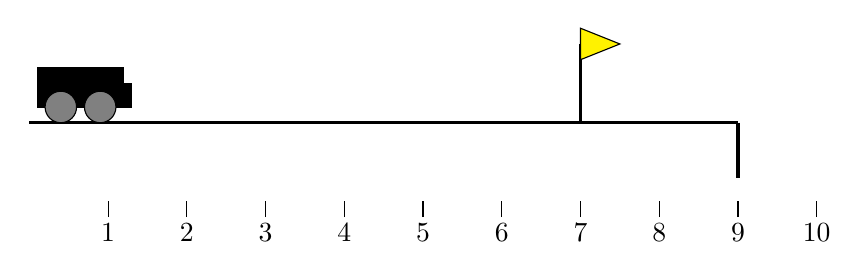
\begin{tikzpicture}

% Ground
\draw[very thick] (0,0) -- (9,0);

% Tick marks and labels
\foreach \x in {1,...,10} {
  \draw (\x,-1.2) -- (\x,-1);
  \node at (\x,-1.4) {\x};
}

% Cliff
\draw[very thick] (9,0) -- (9,-0.7);

% Flag pole
\draw[thick] (7,0) -- (7,1);

% Flag
\draw[fill=yellow] (7,0.8) -- (7.5,1) -- (7,1.2) -- cycle;

% Car body
\draw[fill=black] (0.1,0.2) rectangle (1.2,0.7);
\draw[fill=black] (0.1,0.2) rectangle (1.3,0.5);

% Car wheels
\draw[fill=gray] (0.4,0.2) circle (0.2cm);
\draw[fill=gray] (0.9,0.2) circle (0.2cm);

\end{tikzpicture}
\end{center}

Assume that $\gamma \in [0, 1)$, 
all rewards are bounded, 
the Q-values are initialized to 0, and $\alpha_t = \frac{1}{t+1}$. Transitions are deterministic.

\begin{subparts}

\subpart[2] \textbf{Short Answer:}  Neural uses tabular Q-learning to find $Q^*(s,a)$ for every state and action, and he runs 10,000 iterations. Neural claims that if he randomly chooses the initial state of the car at the start of each iteration and randomly selects each action, then he is guaranteed to converge to $Q^*(s,a)$ by the end of the training run. Is Neural's claim correct? Briefly justify your answer in 1-2 sentences.
    \fillwithlines{7em}
    \begin{soln} 
        Q is only guaranteed to converge to $Q^*$ if each (state, action) pair is also visited infinitely often. In this case, finite iterations and random state initialization makes it possible that some states are never visited at all.
    \end{soln}
    \begin{qauthor}
        Max, Identify the conditions under which the Q-learning algorithm will converge to the true value function
    \end{qauthor}

    % Sort of gives away the answer to the previous question.
    %
    % \subpart[2] \textbf{Short Answer:} Markov decides to run an infinite number of iterations, but at the start of each iteration, Markov always chooses an initial state with a position that is strictly to the left of the previous initial state. The position of the initial state in the first iteration is 10 (the flag). Is Markov guaranteed to converge to $Q^*(s,a)$? Briefly justify your answer in 1-2 sentences.\\ 
    % \fillwithlines{7em}
    % \begin{soln} 
    %     Yes, now every state is visited infinitely often, and the order in which states are visited doesn't matter in Q-learning.
    % \end{soln}
    % \begin{qauthor}
    %     Max, Identify the conditions under which the Q-learning algorithm will converge to the true value function
    % \end{qauthor}

\uplevel{For the questions below, the current state is $s$, the policy takes action $a$ and receives reward $r$, and transitions to state $s'$.}


\subpart[1] \textbf{Numerical answer:} For tabular $Q$-learning with this environment, how many table entries are there in the table $Q$?
    \begin{tcolorbox}[fit,height=1cm, width=4cm, blank, borderline={1pt}{-2pt}]
    %solution
    \end{tcolorbox}
    \begin{soln}
    200
    \end{soln}
    \begin{qauthor}
    Matt
    \end{qauthor}

\subpart[2] \textbf{Numerical answer:} Suppose the car is in state $s = (p=5, v=2)$ and the agent takes action `do nothing' so that we end in state $s'= (p=7, v=1)$ and receive reward $r=8$. Assume $\gamma$ is $0.5$. Suppose (for this problem only) that all $Q$ table entries were initialized to $4$. The Q-learning update rule would update one table entry. What is its new value?
    \begin{tcolorbox}[fit,height=1cm, width=4cm, blank, borderline={1pt}{-2pt}]
    %solution
    \end{tcolorbox}
    \begin{soln}
    $8 + 0.5 * 4 = 10$
    \end{soln}
    \begin{qauthor}
    Matt
    \end{qauthor}

\clearpage

\subpart[2] Consider applying two variants of Q-learning to this problem:
\begin{enumerate}
    \item[(A)] Apply the Q-learning update rule to a random past $(s, a, r, s')$ tuple and then randomly select the next action via $\epsilon$-greedy. Repeat.
    \item[(B)] Randomly select the next action via $\epsilon$-greedy and then immediately apply the Q-learning update rule to the current $(s, a, r, s')$. Repeat.
\end{enumerate}
\textbf{True or False:} In practice, variant (A) is unlikely to yield a better policy than variant (B) because environment is deterministic. \textbf{Briefly justify your answer.}
    \begin{checkboxes}
     \choice True 
     \choice False
    \end{checkboxes}
    \fillwithlines{8em}
    \begin{soln}
    False. Variant (A) is uniform experience reply which is likely to help because of the delayed/infrequent positive rewards.
    \end{soln}
    \begin{qauthor} Matt    \end{qauthor}

\subpart[2] \textbf{Select all that apply:} Now suppose the environment uses a stochastic transition distribution and stochastic rewards that simulate a Pittsburgh winter by allowing the car to randomly slip an extra position to the right at icy positions. Why would it be unwise to use the Q-learning update rule?
\begin{align*}
    Q(s,a) \gets r + \gamma \max_{a' \in \Ac} Q(s', a')
\end{align*}
    {%
    \checkboxchar{$\Box$} \checkedchar{$\blacksquare$} % change checkbox style locally
    \begin{checkboxes}
     \choice the current state $s$ might not be representative of the expected state $s$ at a given timestep in the trajectory
     \choice the action $a$ might not be representative of the most probable action under the $\epsilon$-greedy policy
     \choice the reward $r$ might not be representative of expected reward for the current $(s,a)$ pair
     \choice the next state $s'$ might not be representative of the most probable next state for the current $(s,a)$ pair
     \choice None of the above
    \end{checkboxes}
    }
    \begin{soln}
    C. and D. 
    \end{soln}
    \begin{qauthor}Matt
    \end{qauthor}
    
\end{subparts}


\part[1] \textbf{True or False:} If the state transition distribution and reward function are unknown, Q-learning cannot be used to learn a policy, but deep Q-learning can be applied.
    \begin{checkboxes}
     \choice True 
     \choice False
    \end{checkboxes}
    \begin{soln}
    False. Q learning and deep Q-learning can both be applied in this setting.
    \end{soln}
    \begin{qauthor}
    Matt
    \end{qauthor}


\part[1] \textbf{Fill in the blank by selecting one:} \textit{Deep Q-learning defines a neural network to approximate \underline{\hspace{8em}} which is helpful for very large \underline{\hspace{8em}} space(s)?}
    \begin{checkboxes}
     \choice $V(s)$  / state 
     \choice $V(s)$  / action 
     \choice $V(s)$  / state and action 
     \choice $Q(s,a)$ / state 
     \choice $Q(s,a)$ / action
     \choice $Q(s,a)$ / state and action
    \end{checkboxes}
    \begin{soln}
    $Q(s,a)$ / state
    
    TODO: rewrite this question since "action" and "state and action" are also perfectly valid answers
    \end{soln}
    \begin{qauthor}Matt
    \end{qauthor}

\end{parts}
\clearpage
\input{qs-PCA.tex}
\clearpage
\sectionquestion{$k$-Means}

\begin{parts}

\part[2] \textbf{Select all that apply:} Which of the following statements about optimizing the K-means objective function is correct? \\
    {%
    \checkboxchar{$\Box$} \checkedchar{$\blacksquare$} % change checkbox style locally
    \begin{checkboxes}
     \choice Both gradient descent and coordinate descent can be used to optimize the K-means objective function.
     \choice The K-means objective function is convex so gradient descent is guaranteed to always find the optimal clustering.
     \choice Because block coordinate descent does not optimize all of the variables simultaneously, the objective function's value can increase from iteration to iteration.
     \choice The optimal clustering that minimizes the K-means objective function can be solved for in closed form but doing so is computational expensive. 
     \choice None of the above
    \end{checkboxes}
    }
    \begin{soln}
        None of the above
    \end{soln}
    \begin{qauthor}
        Max Tang, Connect the nonconvexity of the K-Means objective function with the (possibly) poor performance of random initialization

        Lightly edited by Henry
    \end{qauthor}

\part Honk and Chonk are having a clustering competition! They both start with the same dataset of unlabelled data points, $\mathcal{D}$, and they agree to both use K-means with $K=3$. Honk decides to use Lloyd's method, the version of the algorithm presented in lecture where the cluster centers are initialized to randomly selected data points in $\mathcal{D}$. Chonk decides to use block coordinate descent as well except instead of initializing the cluster centers, he initializes the \emph{cluster assignments} by randomly choosing an integer from ${1,2,3}$ for each data point in $\mathcal{D}$.

\begin{subparts}
    \subpart[2] \textbf{True or False:} Both Honk and Chonk's clustering algorithms will always return $3$ clusters of points. Briefly justify your answer in 1-2 concise sentences. 
    \begin{checkboxes}
         \choice True 
         \choice False
    \end{checkboxes}
    \fillwithlines{8em}
    \begin{soln}
        False, Chonk's algorithm could initialize one of the clusters to be empty e.g., no data point is assigned to cluster 3 at initialization. If this is the case, the algorithm will only return 2 clusters. 
    \end{soln}
    \begin{qauthor}
        Henry
    \end{qauthor}

    \clearpage
    \subpart[2] \textbf{True or False:} Despite their different initialization methods, Honk and Chonk's clustering algorithms \emph{could} converge to the same final clustering. Briefly justify your answer in 1-2 concise sentences. 
    \begin{checkboxes}
         \choice True 
         \choice False
    \end{checkboxes}
    \fillwithlines{8em}
    \begin{soln}
        True, if after some number of iterations, both algorithms have the same assignments and cluster centers, then every subsequent iteration of block coordinate descent will behave identically and the two will return the same final clustering. 
    \end{soln}
    \begin{qauthor}
        Henry
    \end{qauthor}

\begin{EnvFullwidth}
    Neural decides to enter the competition but because he has taken 10-301/601, he decides to use K-means++ to initialize his block coordinate descent algorithm. 
\end{EnvFullwidth}
    
    \subpart[2] \textbf{True or False:} Neural's clustering at convergence is guaranteed to have a lower objective function value than both Honk and Chonk's clusterings at convergence. Briefly justify your answer in 1-2 concise sentences. 
    \begin{checkboxes}
         \choice True 
         \choice False
    \end{checkboxes}
    \fillwithlines{8em}
    \begin{soln}
        False, because all of these initialization methods have some randomness, we cannot guarantee that K-means++ will outperform either of the other two e.g., there is some non-zero probability that both Neural and Honk initialize their algorithms to the same set of cluster centers, in which case they will both return the same final clustering. 
    \end{soln}
    \begin{qauthor}
        Henry
    \end{qauthor}
\end{subparts}

\end{parts}
\clearpage
\sectionquestion{Ensemble Methods}

\begin{parts}
    \part Professor Oak trains a random forest consisting of 3 decision trees, $\{t_1, t_2, t_3\}$, on a binary classification dataset with 5 data points. He sends Professor Elm the following table, that summarizes which data points were used to train each decision tree as well as what each decision tree would predict on the individual data points: 
    \begin{center}
        \begin{tabular}{c c|c c c|c c c} 
            & & Used to & Used to & Used to & & & \\
            $i$ & Label & train $t_1$ & train $t_2$ & train $t_3$ & $t_1(x^{(i)})$ & $t_2(x^{(i)})$ & $t_3(x^{(i)})$ \\ \hline
            1 & + & \checkmark & \checkmark & & + & - & + \\ 
            2 & - & & \checkmark & & - & - & - \\ 
            3 & - & \checkmark & & \checkmark & - & + & - \\ 
            4 & + & \checkmark & & & - & + & + \\ 
            5 & + & & & \checkmark & - & - & + \\ 
            \hline
        \end{tabular}
    \end{center}

    \begin{subparts}
        \subpart[1] \textbf{Numerical answer:} What is the training error rate of Professor Oak's random forest? Break ties in majority votes in favor of the + label. Express your answer as a simplified fraction. 
        \begin{tcolorbox}[fit,height=1cm, width=2cm, blank, borderline={1pt}{-2pt}]
            \begin{soln}
                $\frac{1}{5}$
            \end{soln}
        \end{tcolorbox}
        
        \subpart[1] \textbf{Numerical answer:} What is the out-of-bag error rate of Professor Oak's random forest? Break ties in majority votes in favor of the + label. Express your answer as a simplified fraction. 
        \begin{tcolorbox}[fit,height=1cm, width=2cm, blank, borderline={1pt}{-2pt}]
            \begin{soln}
                $\frac{2}{5}$
            \end{soln}
        \end{tcolorbox}
    \end{subparts}
    
    \begin{qauthor}
        Henry
    \end{qauthor}
    
    \part[2] \textbf{Select all that apply:} Suppose you run the weighted majority algorithm with two linear decision boundaries, $h_1$ and $h_2$, as your initial classifiers and you learn classifier weights $\alpha_1$ and $\alpha_2$. Assuming sign$(0)=+1$, which of the following conditions \emph{could} result in the learned ensemble having a non-linear decision boundary? 
    {%
    \checkboxchar{$\Box$} \checkedchar{$\blacksquare$} % change checkbox style locally
    \begin{checkboxes}
     \choice $h_1$ and $h_2$ are not parallel \emph{and} $\alpha_1 \ne \alpha_2$
     \choice $h_1$ and $h_2$ are not parallel \emph{and} $\alpha_1 = \alpha_2$
     \choice $h_1$ and $h_2$ are parallel \emph{and} $\alpha_1 \ne \alpha_2$
     \choice $h_1$ and $h_2$ are parallel \emph{and} $\alpha_1 = \alpha_2$
     \choice None of the above
    \end{checkboxes}
    }
    \begin{soln}
        B, D
    \end{soln}
    \begin{qauthor}
        Henry
    \end{qauthor}

\clearpage
    \part[2] \textbf{Drawing:} The figure below shows a set of linear decision boundaries and the corresponding weights learned using the weighted majority algorithm; the colored arrow matching each decision boundary corresponds to the side that each classifier predicts as positive. 

    \begin{center}
        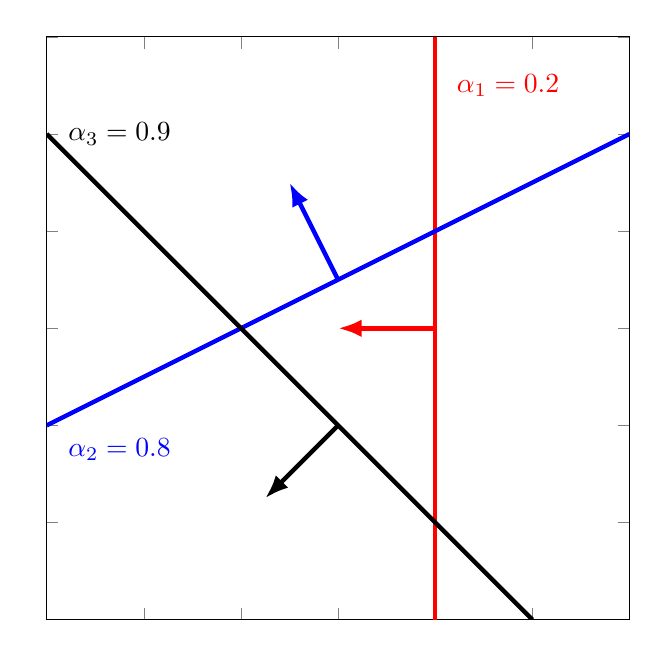
\begin{tikzpicture}
        \begin{axis}[
            scale=1.3, axis equal image, mark options={scale=1.5},
            xmin=0, xmax=6, xtick={}, xticklabel=\empty,
            ymin=0, ymax=6, ytick={}, yticklabel=\empty,
            samples=50]
            \addplot[red, ultra thick] coordinates { (4, 0) (4, 6) };
            \node[red] at (4.75, 5.5) {$\alpha_1 = 0.2$};
            \addplot[blue, ultra thick] coordinates { (6, 5) (0, 2) };
            \node[blue] at (0.75, 1.75) {$\alpha_2 = 0.8$};
            \addplot[black, ultra thick] coordinates { (5, 0) (0, 5) };
            \node[black] at (0.75, 5) {$\alpha_3 = 0.9$};
            \draw [-{Latex[length=3mm]}, red, ultra thick] (4,3) -- (3,3);
            \draw [-{Latex[length=3mm]}, blue, ultra thick] (3,3.5) -- (2.5,4.5);
            \draw [-{Latex[length=3mm]}, black, ultra thick] (3,2) -- (2.25,1.25);
        \end{axis}
        \end{tikzpicture} 
    \end{center}

    On the figure, lightly shade the area(s) that would be classified as positive by the ensemble formed using these decision boundaries and weights. 
    
    \begin{soln}
        \begin{center}
            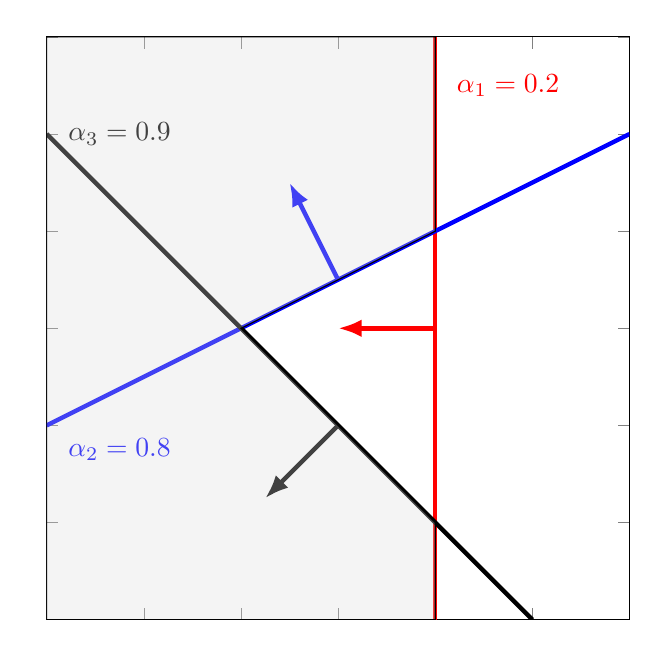
\begin{tikzpicture}
            \begin{axis}[
                scale=1.3, axis equal image, mark options={scale=1.5},
                xmin=0, xmax=6, xtick={}, xticklabel=\empty,
                ymin=0, ymax=6, ytick={}, yticklabel=\empty,
                samples=50]
                \addplot[red, ultra thick] coordinates { (4, 0) (4, 6) };
                \node[red] at (4.75, 5.5) {$\alpha_1 = 0.2$};
                \addplot[blue, ultra thick] coordinates { (6, 5) (0, 2) };
                \node[blue] at (0.75, 1.75) {$\alpha_2 = 0.8$};
                \addplot[black, ultra thick] coordinates { (5, 0) (0, 5) };
                \node[black] at (0.75, 5) {$\alpha_3 = 0.9$};
                \draw [-{Latex[length=3mm]}, red, ultra thick] (4,3) -- (3,3);
                \draw [-{Latex[length=3mm]}, blue, ultra thick] (3,3.5) -- (2.5,4.5);
                \draw [-{Latex[length=3mm]}, black, ultra thick] (3,2) -- (2.25,1.25);
                \draw [fill=gray!30, fill opacity=0.3] (0, 0) -- (0, 6) -- (4, 6) -- (4, 4) -- (2, 3) -- (4, 1) -- (4, 0) -- cycle;
            \end{axis}
            \end{tikzpicture} 
        \end{center}
    \end{soln}
    

    \part[1] \textbf{Numerical answer:} While running AdaBoost, Neural observes that the weights on all of his data points do not change from iteration $t$ to iteration $t+1$, i.e., $D_{t+1}(i) = D_t(i)$ $\forall$ $i$, regardless of whether or not they were multiplied by $\exp(-\alpha_t)$ or $\exp(\alpha_t)$ where $\alpha_t = \frac{1}{2}\ln \frac{1-\epsilon_t}{\epsilon_t}$. What was $\epsilon_t$, the weighted training error of the weak learner in the $t^{\textrm{th}}$ iteration?
    
    \begin{tcolorbox}[fit,height=1cm, width=2cm, blank, borderline={1pt}{-2pt}]
        \begin{soln}
            $\frac{1}{2}$
        \end{soln}
    \end{tcolorbox}
    \begin{qauthor}
        Henry
    \end{qauthor}
\end{parts}
\clearpage
\sectionquestion{Recommender Systems}

\begin{parts}

\part Neural the Narwhal asks his friends (6 users) to rate their favorite sea animals (8 items). He has a sparse ratings matrix of size $6 \times 8$, and he wants to use collaborative filtering to factor this matrix into a user matrix and an item matrix.

\begin{subparts}

    \subpart[2] \textbf{Select All That Apply:}  He thinks, since each latent feature captures information about the underlying data, he wants to factor the user matrix $\Uv$ into size $6 \times 10000$ and the item matrix $\Vv$ into size $8 \times 10000$. Is Neural's choice of $10000$ latent features a reasonable decision?
    {%
    \checkboxchar{$\Box$} \checkedchar{$\blacksquare$} % change checkbox style locally
    \begin{checkboxes}
     \choice Yes, because more latent features are able to capture more data about the factors that go into the ratings, thus leading to model that generalizes better.
     \choice Yes, because after these matrices are learned, predictions will be made on new users, causing the user matrix to grow.
     \choice No, because the matrices that are learned may overfit on the dataset.
     \choice No, because the matrix cannot be factored at all unless the number of latent features is $\min(6,8)$.
     \choice None of the above
    \end{checkboxes}
    }
    \begin{soln}
    C
    \end{soln}
    \begin{qauthor}
    Emily (edited by Matt), Recommender Systems\\
    AFTER FEEDBACK: took by taking out line saying that Neural is wrong and reword question to not imply if this is a good or bad method. changed short answer into select all that apply options.
    \end{qauthor}

    \uplevel{Neural now tries using only 2 features in the latent space, so the user matrix $\Uv$ is of size $6 \times 2$ and so the item matrix $\Vv$ is of size $8 \times 2$.
    Suppose an oracle provides a new user vector $\uv_i \in \Rb^2$, i.e. with 2 latent features. }

    \subpart[1] \textbf{Mathematical answer:} 
    Write an expression to predict the rating given to the $j$ item (sea animal) by the new user vector $\uv_i$.
    \begin{tcolorbox}[fit,height=2cm, width=7cm, blank, borderline={1pt}{-2pt}]
    %solution
    \end{tcolorbox}
    \begin{soln}
    $\uv_i^T \Vv_{j,\cdot}$
    \end{soln}
    \begin{qauthor}
    Matt
    \end{qauthor}
    
    \subpart[2] \textbf{Mathematical answer:} 
    Write an expression to predict \textit{which} item (sea animal) the user will rate the highest; this integer is the recommendation to the user.
    (Hint: you may use the $\argmax$ function to obtain the index of the maximum value in a vector or matrix.)
    \begin{tcolorbox}[fit,height=2cm, width=7cm, blank, borderline={1pt}{-2pt}]
    %solution
    \end{tcolorbox}
    \begin{soln}
    $\texttt{argmax}(\uv_i V^T)$
    \end{soln}
    \begin{qauthor}
    Emily, Recommender Systems
    \end{qauthor}
    \begin{qtester}
    Somewhat open-ended with how Neural is wrong in part a -- students may end up saying ``predictions aren't guaranteed to be good even with all important features'' or something similar. The goal of the question seems to be getting at matrix factorization as an approximation/a low dimensional projection of users and items. The matrices Neural could find could simply reconstruct the original matrix exactly, which may make the question's discussion of ``every important feature'' confusing.

    Part b looks fine.
    \end{qtester}
    
\end{subparts}

\end{parts}


\clearpage
\sectionquestion{Miscellaneous}

\begin{parts}

\part[1] \textbf{Short answer:} Describe \textbf{one} topic \textbf{in detail} from the course material \textbf{in Lectures 17 - 25} that was \textbf{not covered on the exam}. For example, a learning objective that you reviewed that was not asked about here, a comparison of two algorithms or ML methods, etc. Write your answer in \textbf{3-5 sentences}.
\fillwithlines{18em}
\begin{soln}
    Accept pretty much anything that satisfies the above conditions.
\end{soln}
\begin{qauthor}
    Matt
\end{qauthor}
    
\end{parts}
    

\clearpage
\end{questions}

% DO NOT COMMENT THIS SECTION OUT!! -Matt
\clearpage
\begin{center}
Do not remove this page! Use this page for scratch work.
\end{center}
\clearpage
\begin{center}
Do not remove this page! Use this page for scratch work.
\end{center}
\clearpage
\begin{center}
Do not remove this page! Use this page for scratch work.
\end{center}
\clearpage
\begin{center}
Do not remove this page! Use this page for scratch work.
\end{center}
\clearpage
\begin{center}
Do not remove this page! Use this page for scratch work.
\end{center}
\end{document}
